\documentclass[a4,10pt]{aleph-notas}

% -- Paquetes adicionales
\usepackage{enumitem}
\usepackage{aleph-comandos}
\usepackage{quantikz}

% -- Datos
\institucion{Proyecto Alephsub0}
\asignatura{Computación Cuántica}
\tema{Algoritmo de Deutsch}
\autor{Andrés Merino}
\fecha{Agosto 2026}

\fuente{montserrat}
\logouno[4.5cm]{Logos/LogoAlephsub0-02}
\definecolor{colordef}{cmyk}{0.81,0.62,0.00,0.22}

% -- Comandos adicionales
\newtheorem*{prob}{Problema}
    \tcolorboxenvironment{prob}{%
        color=colordef,recuadrost,colback=colordef!7,drop fuzzy shadow
    }

\begin{document}


\encabezado

El algoritmo de Deutsch permite determinar, con una sola consulta a un oráculo cuántico, si una función booleana
\[
    f:\{0,1\}\longrightarrow\{0,1\}
\]
es constante o balanceada. La función es \emph{constante} si \(f(0)=f(1)\), y es \emph{balanceada} si \(f(0)\neq f(1)\).

La idea es:
\begin{itemize}
    \item Se preparan dos cúbits en el estado \(\ket{0}\ket{1}\).
    \item Se aplica la compuerta Hadamard a ambos cúbits para crear una superposición de las dos posibles entradas de \(f\).
    \item Se consulta una sola vez el oráculo cuántico \(U_f\), definido por
    \[
        U_f\ket{x}\ket{y}=\ket{x}\ket{y\oplus f(x)},
    \]
    con $x,y\in\{0,1\}$ y donde \(\oplus\) representa la suma módulo \(2\).
    \item Gracias al retroceso de fase, los valores \(f(0)\) y \(f(1)\) quedan codificados en la fase relativa del primer cúbit.
    \item Después de aplicar otra compuerta Hadamard al primer cúbit, su medición produce \(0\) si \(f\) es constante y \(1\) si es balanceada.
\end{itemize}

El circuito del algoritmo de Deutsch es:
\begin{center}
    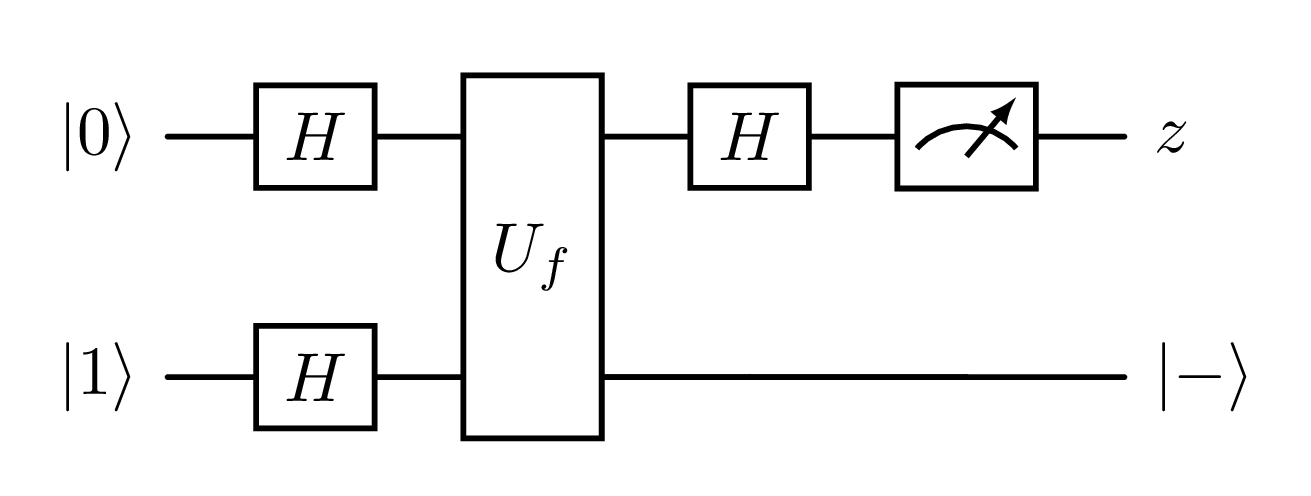
\includegraphics[width=0.65\textwidth]{imagen.png}
\end{center}

\begin{prob}
    Realizar la derivación matemática del algoritmo de Deutsch y demostrar que permite distinguir con certeza si \(f\) es constante o balanceada mediante una sola consulta al oráculo \(U_f\).
\end{prob}

\begin{proof}
    Sean \(q_0\) y \(q_1\) los cúbits de entrada y auxiliar, respectivamente. El estado inicial del sistema es
    \[
        \ket{\Psi_0}=\ket{0}\ket{1}.
    \]

    Consideremos los siguientes pasos del circuito:
    \begin{center}
        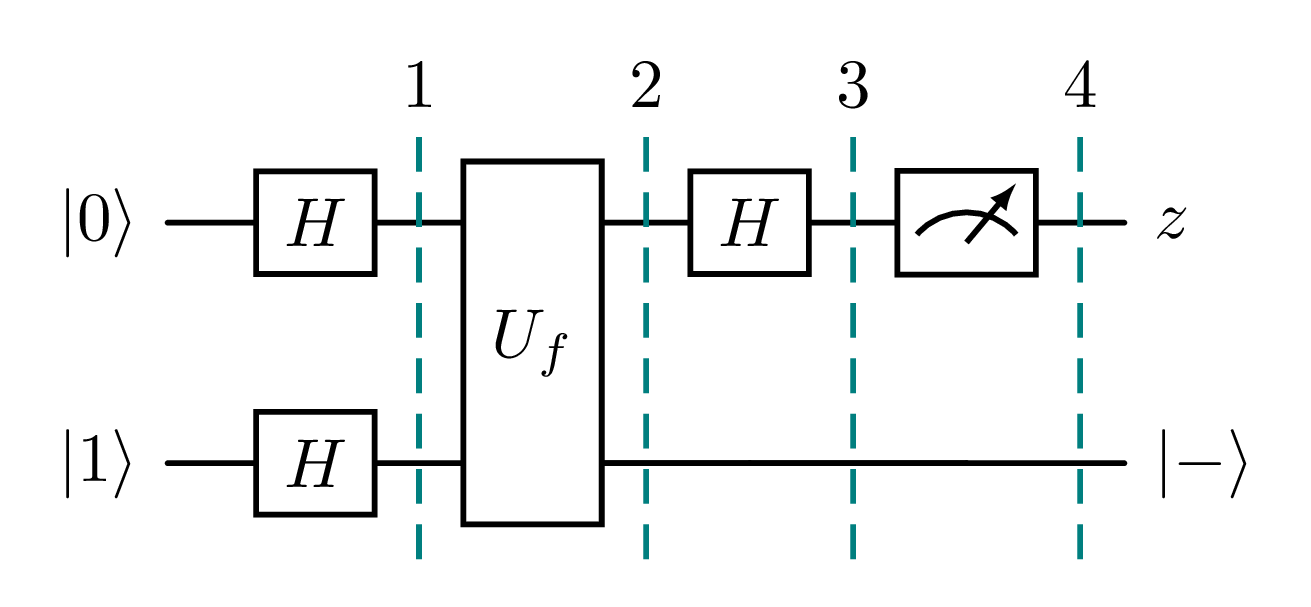
\includegraphics[width=0.65\textwidth]{imagen2.png}
    \end{center}

    \begin{itemize}
        \item \textbf{Paso 1.} Se aplica la compuerta Hadamard a ambos
        cúbits:
        \[
            \ket{\Psi_1}=(H\otimes H)\ket{0}\ket{1}.
        \]
        Puesto que
        \[
            H\ket{0}=\frac{\ket{0}+\ket{1}}{\sqrt{2}}=\ket{+},
            \qquad
            H\ket{1}=\frac{\ket{0}-\ket{1}}{\sqrt{2}}=\ket{-},
        \]
        se obtiene
        \begin{align*}
            \ket{\Psi_1}
            &=\ket{+}\ket{-}\\
            &=\frac{1}{2}
            \left(\ket{00}-\ket{01}+\ket{10}-\ket{11}\right).
        \end{align*}
        En particular, el primer cúbit representa simultáneamente las dos entradas posibles, \(x=0\) y \(x=1\).

        \item \textbf{Paso 2.} Se aplica el oráculo \(U_f\). Para cada \(x\in\{0,1\}\), su acción sobre el segundo cúbit es
        \begin{align*}
            U_f\bigl(\ket{x}\ket{-}\bigr)
            &=\frac{1}{\sqrt{2}}
            \left(\ket{x}\ket{f(x)}
            -\ket{x}\ket{1\oplus f(x)}\right)\\
            &=(-1)^{f(x)}\ket{x}\ket{-}.
        \end{align*}
        Así, el valor de la función se transfiere a la fase del primer cúbit, mientras el segundo permanece en \(\ket{-}\). Este fenómeno se denomina \emph{retroceso de fase}. Por tanto,
        \begin{align*}
            \ket{\Psi_2}
            &=U_f\ket{\Psi_1}\\
            &=\frac{1}{\sqrt{2}}
            \left(
                (-1)^{f(0)}\ket{0}
                +(-1)^{f(1)}\ket{1}
            \right)\ket{-}.
        \end{align*}

        \item \textbf{Paso 3.} Se aplica nuevamente la compuerta Hadamard al primer cúbit. Como
        \[
            H\ket{0}=\frac{\ket{0}+\ket{1}}{\sqrt{2}},
            \qquad
            H\ket{1}=\frac{\ket{0}-\ket{1}}{\sqrt{2}},
        \]
        resulta
        \begin{align*}
            \ket{\Psi_3}
            &=(H\otimes I)\ket{\Psi_2}\\
            &=\frac{1}{2}\Bigl[
                \bigl((-1)^{f(0)}+(-1)^{f(1)}\bigr)\ket{0}\\
            &\hspace{3.4cm}
                +\bigl((-1)^{f(0)}-(-1)^{f(1)}\bigr)\ket{1}
            \Bigr]\ket{-}.
        \end{align*}

        Analicemos las dos posibilidades:
        \begin{itemize}
            \item Si \(f\) es constante, entonces \(f(0)=f(1)\). El coeficiente de \(\ket{1}\) es cero y
            \[
                \ket{\Psi_3}=(-1)^{f(0)}\ket{0}\ket{-}.
            \]
            El factor \((-1)^{f(0)}\) es una fase global y no altera el resultado de una medición.

            \item Si \(f\) es balanceada, entonces \(f(0)\neq f(1)\). El coeficiente de \(\ket{0}\) es cero y
            \[
                \ket{\Psi_3}=(-1)^{f(0)}\ket{1}\ket{-}.
            \]
            Nuevamente, el signo global no tiene consecuencias observables.
        \end{itemize}

        \item \textbf{Paso 4.} Finalmente, se mide el primer cúbit en la base computacional. El resultado es
        \[
            \begin{array}{c|c}
                \text{Resultado} & \text{Tipo de función}\\
                \hline
                0 & f\text{ es constante}\\
                1 & f\text{ es balanceada}
            \end{array}
        \]
        y se obtiene con probabilidad \(1\) en ambos casos.
    \end{itemize}

    En consecuencia, el algoritmo de Deutsch distingue con certeza si \(f\) es constante o balanceada utilizando una sola consulta a \(U_f\). En un procedimiento clásico determinista, en cambio, es necesario evaluar tanto \(f(0)\) como \(f(1)\), es decir, realizar dos consultas en el peor caso.
\end{proof}




\end{document}
